% =================================================================
% CS-412 Fuzzing Lab — Report Template (USENIX format)
%=================================================================
\documentclass[letterpaper,twocolumn,10pt]{article}
\usepackage{usenix-2020-09}
\usepackage{graphicx}
\usepackage{booktabs}
\usepackage{listings}
\usepackage{hyperref}
\usepackage{xcolor}
\usepackage{tabularx}
\usepackage{enumitem}


\lstset{
  basicstyle=\footnotesize\ttfamily,
  breaklines=true,
  frame=single,
  language=C,
  numbers=left,
  numberstyle=\tiny\color{gray},
  captionpos=b
}
\raggedbottom


\begin{document}

\title{Software Security CS-412: Fuzzing Lab Report:\\Fuzzing libpng 1.2.27}

\author{
  {\rm Dominique Sheng Huang}\\EPFL
  \and
  {\rm Tinghong Jin}\\EPFL
  \and
  {\rm Menghan Li}\\menghan.li@epfl.ch
  \and
  {\rm Shunchang Liu}\\EPFL
}

\maketitle

% -----------------------------------------------------------------
% Q1 — Harness Design
% -----------------------------------------------------------------
% 插入harness代码-引用？See Listing~\ref{lst:harness} in the appendix for the full harness source code.

\section{Harness Design}
\label{sec:q1}
\paragraph{Entry Point Choice:}~\\[0.3em]
We chose a set of Low-level Decoder \& Transformation APIs as our entry point. For example, after reading the metadata with \texttt{png\_read\_info}, we used a customized \texttt{run\_png\_set} function to invoke different combinations of the \texttt{png\_set\_*} family functions (such as \texttt{png\_set\_dither}, \texttt{png\_set\_gamma}, \texttt{png\_set\_rgb\_to\_gray}, etc.) to alter the decoder's state. Subsequently, we allocate the appropriate memory space and read the image data using \texttt{png\_read\_image()}.\\[0.3em]
\textbf{Analysis:} In real-world scenarios, image libraries mostly receive untrusted input, thus making the decoder a relatively large attack surface. Furthermore, our rationale for creating a customized function to invoke different combinations of \texttt{png\_set\_*} functions is that libpng vulnerabilities do not solely exist in header parsing. Rather, they often lie within the various combinations of complex image transformation logic. Therefore, the core logic of our customized transformation calls is using the first 16 bytes of the input file as a ``Configuration'' to generate a call sequence(combination) for the \texttt{png\_set\_*} APIs. This enables AFL to explore deeper paths within libpng and trigger branches that increase code coverage.


\paragraph{Alternatives:}~\\


\paragraph{Data-Flow of Harness (persistent) code:}In our Harness code design, the data flow from AFL++ to the libpng API is as follows:
\begin{itemize}[leftmargin=*]
    \item Get input: The test cases generated by AFL are first loaded into the pointer \texttt{buf}, and then divided into two parts: the first 16 bytes are extracted into \texttt{config}, and the remaining bytes are the PNG image payload.
    \item Handle I/O: We created a custom memory read callback, \texttt{png\_read\_callback\_fn}, using \texttt{png\_set\_read\_fn}. The \texttt{read\_handle} structure stores the memory address and size of the PNG payload.
    \item Get Metadata: Then, call \texttt{png\_read\_info} to pull data from \texttt{buf}, parse header information such as IHDR, and obtain the original width, height and color type, etc.
    \item Customized Transformation combination: Next, we receive the first 16 bytes of configuration data \texttt{config} through the custom \texttt{run\_png\_set}, and generate flags and their corresponding values based on them. Different flag values correspond to different transformation function APIs, so each time AFL mutates these configuration bytes, different \texttt{png\_set\_*} functions will be triggered.
    \item Read data: Finally, call \texttt{png\_read\_update\_info} to update the converted image information, then allocate memory and call \texttt{png\_read\_image} to write the pixel data into the allocated \texttt{row\_pointers} buffer.
\end{itemize}


\paragraph{Guards Explanation:} Each Guard in the code is designed to minimize false positives generated by fuzzing, thus preventing waste of control flow and resources.
\begin{itemize}[leftmargin=*]
    \item \texttt{if (len <= CONFIG\_SIZE)}: Ensure the input is long enough to extract the 16-byte configuration; otherwise, direct extraction will result in an OOB Read, leading to false positives.
    \item \texttt{if (!png) ... if (!info)}: Prevent basic memory allocation failures.
    \item \texttt{if (setjmp(png\_jmpbuf(png)))}: Error capture mechanism. When libpng encounters an malformed PNG, it calls \texttt{longjmp} to terminate the process directly. If this isn't captured, AFL will record it as a crash, causing false positives. Capturing it and jumping to \texttt{cleanup} allows the program to handle malformed input stably.
    \item \texttt{if ((size\_t)height > PNG\_SIZE\_MAX / sizeof(png\_bytep))}: too large height?...
    \item \texttt{if ((width == 0) || (height == 0) || (width > PNG\_MAX\_WIDTH) || ...)}: Prevent AFL from generating legally large images. Setting a reasonable threshold (\texttt{PNG\_MAX\_PIXELS}) ensures that CPU and memory resources are focused on exploring code paths, guaranteeing fuzzing throughput.
\end{itemize}




% -----------------------------------------------------------------
% Q2 — Instrumentation and Sanitizers
% --------------------------------------------------------

\section{Instrumentation and Sanitizers}
\label{sec:q2}

\paragraph{Instrumentation \& Flags:}
\begin{itemize}[leftmargin=*]
    \item \texttt{CC=afl-clang-fast / CXX=afl-clang-fast++}: Used in white-box fuzzing. The compilation process calls the afl-clang-fast wrapper, which injects lightweight coverage tracking probes (instrumentaion) at the edges of each basic block in the CFG. If omitted, the fuzzer will not be able to obtain coverage feedback, degenerating into blind/blackbox fuzzing, and AFL will also not be able to know which mutations triggered new paths, resulting in inefficient fuzzing.
    \item \texttt{-fsanitize=address}: This is ASan, which inserts``redzone'' around memory allocation and uses shadow memory to track memory state, in order to catch memory violations such as OOB and UAF at runtime; if omitted, many memory corruptions (such as only one or two bytes heap overflows) will not immediately cause crash, so these may be missed without ASan.
    \item \texttt{-g}: To contains DWARF debugging information (including symbol tables and source code line number mappings) in the compiled binary file . If omitted, when ASan captures a memory corruption or a program crash, crash triage will become difficult without these infos because it's impossible to know which line in which source file the crash occurred.
    \item \texttt{-O1}: Use first-level compiler optimizations to provide a basic performance improvement. If omitted, program execution will be slower, reducing the fuzzer's throughput (executions per second).
    \item \texttt{-fno-omit-frame-pointer}: Used in black-box and noAsan fuzzing. Forces the compiler to keep the frame pointer in the register. If omitted, the generated call stack/backtrace may be broken or missing in QEMU-based black-box fuzzing or when debugging crash cases, making it impossible to trace how the function reached the location.
\end{itemize}

% 引用patch 代码?
\paragraph{Patch:} The patch we used is in file ``changes.patch''.\\
The working principle is to modify the conditional statement originally used to verify the CRC checksum of PNG chunks (from \texttt{crc != png\_ptr->crc} to a logic that always returns false, thereby forcing libpng to ignore all CRC validation errors. Regarding its effect on Path Discovery: since AFL's mutation strategy involves randomly flipping and modifying bytes, the original CRC value will no longer match once AFL alters the chunk. If the patch is omitted, the majority of mutated files will be directly rejected and discarded by libpng early in the parsing process (during the CRC validation phase). Consequently, code coverage would get stuck, preventing the fuzzer from exploring deeper code paths. Removing this check is essential to fully activate AFL's path exploration capabilities.








% -----------------------------------------------------------------
% Q3 — Seed Corpus and Dictionary
% -----------------------------------------------------------------
% 插入屏幕截图并引用，替换量化具体数值等
\section{Seed Corpus and Dictionary}
\label{sec:q3}
\paragraph{Seeds \& Dictionary Description:}~\\[0.3em]
For the seeds, ....\\
For the dictionary, we used the standard AFL PNG dictionary written by Michal Zalewski. This dictionary is specifically tailored to the PNG file format specification. It contains the basic components of a valid PNG file, including the mandatory 8-byte PNG file signature (\texttt{\textbackslash x89PNG\textbackslash x0d\textbackslash x0a\textbackslash x1a\textbackslash x0a}) and various 4-byte ASCII block type identifiers (e.g., IHDR for the header, IDAT for the image data, PLTE for the palette, and other auxiliary blocks such as tEXt or gAMA).

\paragraph{Quantitative Analysis:}
According to the ``fuzzing strategy yields'' section of the AFL++ status screen, we can quantify the contribution of different mutation strategies to code coverage.\\
\textbf{Havoc/Splice Strategy:} The havoc stage contributed the majority of new paths, yielding 1,272 new finds out of approximately 178 million executions (1272/178M). The splice strategy currently yielded 0 finds. Havoc is a highly destructive, multi-pass mutation stage which excels at exploring dense blocks of sequential logic and arithmetic boundaries once a basic code path is unlocked.\\
\textbf{Dictionary Strategy:} The dictionary stage yielded 3 new finds out of roughly 99.6k total executions. Although this is fewer than the 1272 paths above, these dictionary based discoveries are structurally important because the probability of random destructive mutations correctly guessing 4-byte block identifiers like ``PLTE'' is extremely low. The dictionary strategy can effectively bypass these magic byte based bottleneck checks, unlocking new subtrees of the target control flow graph, which facilitates the subsequent discovery of more paths by the destructive mutation strategy.

\paragraph{Formal Terms Explanation:}
Within the framework of formal language/grammar theory, file formats like PNG can be modeled as strings belonging to a specific formal language and constrained by its syntax (e.g., context-free grammars, CFG). Within the CFG-based Fuzzing, entries in our dictionary represent terminal symbols or lexical tokens that constitute the alphabet of that language. When libpng parses an input file, it essentially acts as a pushdown automaton or a complex state machine. It performs lexical analysis to read the input stream and expects specific terminal symbols (e.g., ``IHDR'') to trigger state transitions. Without these precise terminal symbols, the input string is considered syntactically invalid and rejected. Providing a dictionary can transform the fuzzer's behavior from blind and random strings mutation to syntax-aware mutation, enabling the deep semantic parsing logic of the target application.


% -----------------------------------------------------------------
% Q4 — Campaign Analysis
% -----------------------------------------------------------------
\section{Q4 --- Campaign Analysis}
\label{sec:q4}

% TODO (A): Metrics table (stability, corpus, map density, cycles)
% TODO (A): Edges curve interpretation with timestamps
% TODO (A): Saturation argument with evidence
% Reference: see Figure~\ref{fig:status-inst} and Figure~\ref{fig:edges-inst}



% -----------------------------------------------------------------
% Q5 — Crash Triage
% -----------------------------------------------------------------
\section{Q5 --- Crash Triage}
\label{sec:q5}

% TODO (B): Full triage workflow: reproduce → minimize → ASan trace
% TODO (B): Bug type, location, CVE if applicable
% OR: synthetic bug demonstration + argument



% -----------------------------------------------------------------
% Q6 — Attack Surface Analysis
% --------------------------------------------------------
\section{Attack Surface Analysis}
\label{sec:q6}
\paragraph{Application 1: Firefox}~\\[0.3em]
xxx


\paragraph{Application 2: ImageMagick}~\\[0.3em]
ImageMagick is one of the most widely used open-source image processing suites. It is used as the underlying image processing engine by a large number of web frameworks and backend servers (such as PHP, Node.js, etc.), and in its \href{https://github.com/ImageMagick/ImageMagick/blob/main/coders/png.c}{source code} we can check its logic of calling \texttt{libpng}.\\[0.2em]
\textbf{Attack scenario:} Suppose a social media website allows users to upload profile pictures and uses ImageMagick on the backend to crop and resize these images into uniform thumbnails. An attacker creates and uploads a malicious PNG file containing malformed data chunks. When ImageMagick calls \texttt{libpng} to parse the image, the malformed data triggers a Heap Buffer Overflow. The attacker can then exploit this to overwrite function pointers or return addresses on the heap, thereby hijacking the server process's control flow and executing malicious commands on the target server.\\[0.2em]
\textbf{Uncovered path:} In ImageMagick's decoder function, like \texttt{ReadPNGImage} (\texttt{coders/png.c}, line 3911), the core processing involves calling the \texttt{ReadOnePNGImage}  (\texttt{coders/png.c}, line 3968). Within this function, in addition to reading pixel data, it calls numerous \texttt{libpng} data retrieval APIs. For instance, it calls \texttt{png\_get\_iCCP} (line 2553) to read the ICC color profile, and \texttt{png\_get\_text} (line 3657) to read the contents of \texttt{tEXt}/\texttt{zTXt}/\texttt{iTXt} chunks. Although our Harness parses these chunks during the \texttt{png\_read\_info()}, it does not call the relevant \texttt{png\_get\_*} APIs to extract this data to the application layer. Certain memory vulnerabilities might be triggered when the application explicitly requests and copies these malformed decompressed texts or color profile information. Our Harness doesn’t simulate the application layer's behavior of extracting this data, so it may miss such bugs.\\
Similarly, regarding ImageMagick's writing logic in \texttt{WritePNGImage} (\texttt{coders/png.c}, line 11565), the core processing is calling the \texttt{WriteOnePNGImage} (\texttt{coders/png.c}, line 12203). Within this function (line 7977), it calls \texttt{libpng} APIs such as \texttt{png\_create\_write\_struct} (line 9401) and \texttt{png\_write\_info} (line 10908). However, our Harness only conducts read-related testing and does not test the logic involving compression, chunk generation, and writing within \texttt{libpng}. Therefore, bugs occurring during these data output processes (e.g., an integer overflow when calculating chunk lengths during output file generation, leading to a heap overflow) are missed.




% -----------------------------------------------------------------
% Q7 — Binary-Only Fuzzing with QEMU Mode
% -----------------------------------------------------------------
\section{Q7 --- Binary-Only Fuzzing (QEMU)}
\label{sec:q7}

% TODO (C): Side-by-side table: exec speed, edges, corpus
% TODO (C): Explanation of QEMU coverage collection mechanism
% Reference: see Figure~\ref{fig:status-qemu} and Figure~\ref{fig:edges-qemu}



% -----------------------------------------------------------------
% Q8 — Instrumentation Depth and Performance
% -----------------------------------------------------------------
\section{Q8 --- Instrumentation Depth and Performance}
\label{sec:q8}

% TODO (D): Edge count: library-only vs harness binary, explain diff
% TODO (D): Map density vs total edges, explain unreached edges
% TODO (D): 3-config exec speed table + explanations



% =================================================================
%                         APPENDIX
% =================================================================
\appendix

\section{Figures and Screenshots}
\label{app:figures}

% --- Instrumented campaign ---
\begin{figure}[h]
\centering
% \includegraphics[width=\columnwidth]{status_screen_instrumented.png}
\fbox{\parbox{0.9\columnwidth}{\centering\vspace{2em}
  \textit{[A: paste instrumented status screen screenshot here]}
  \vspace{2em}}}
\caption{AFL++ status screen — instrumented campaign (30 min).}
\label{fig:status-inst}
\end{figure}

\begin{figure}[h]
\centering
% 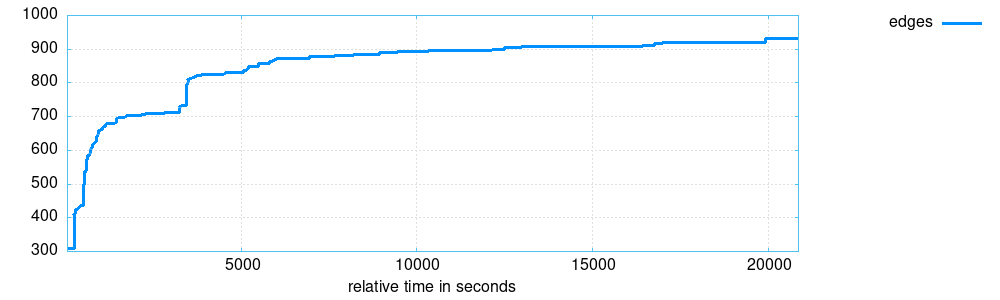
\includegraphics[width=\columnwidth]{plot_output/edges.png}
\fbox{\parbox{0.9\columnwidth}{\centering\vspace{2em}
  \textit{[A: paste edges.png from plot\_output/ here]}
  \vspace{2em}}}
\caption{Edge discovery over time — instrumented campaign.}
\label{fig:edges-inst}
\end{figure}

% --- QEMU campaign ---
\begin{figure}[h]
\centering
% \includegraphics[width=\columnwidth]{status_screen_qemu.png}
\fbox{\parbox{0.9\columnwidth}{\centering\vspace{2em}
  \textit{[C: paste QEMU status screen screenshot here]}
  \vspace{2em}}}
\caption{AFL++ status screen — QEMU campaign (30 min).}
\label{fig:status-qemu}
\end{figure}

\begin{figure}[h]
\centering
% 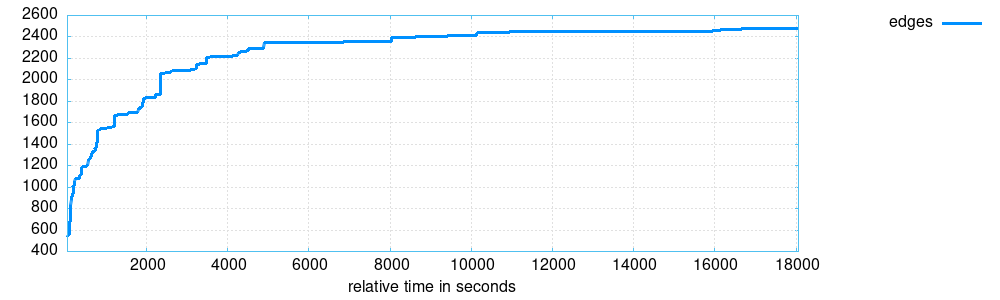
\includegraphics[width=\columnwidth]{plot_output_qemu/edges.png}
\fbox{\parbox{0.9\columnwidth}{\centering\vspace{2em}
  \textit{[C: paste edges.png from plot\_output\_qemu/ here]}
  \vspace{2em}}}
\caption{Edge discovery over time — QEMU campaign.}
\label{fig:edges-qemu}
\end{figure}

% --- ASan trace ---
\begin{figure}[h]
\centering
\fbox{\parbox{0.9\columnwidth}{\centering\vspace{2em}
  \textit{[B: paste ASan stack trace output here]}
  \vspace{2em}}}
\caption{ASan stack trace for the triaged crash.}
\label{fig:asan-trace}
\end{figure}



\section{Code Listings}
\label{app:code}

\begin{figure*}[h]
\begin{lstlisting}[caption={Fuzzing harness (src/harness.c) — excerpt},
                   label={lst:harness}]
/* TODO: paste key sections of harness.c here */
\end{lstlisting}
\end{figure*}


% \begin{figure*}[h]
% \begin{lstlisting}[caption={Patch (changes.patch)},
%                    label={lst:harness}]
% --- libpng-1.2.27/pngrutil.c	2008-04-30 12:23:13.000000000 +0200
% +++ libpng-1.2.27_new/pngrutil.c	2026-05-09 19:02:13.271050837 +0200
% @@ -165,7 +165,10 @@
%     if (need_crc)
%     {
%        crc = png_get_uint_32(crc_bytes);
% -      return ((int)(crc != png_ptr->crc));
% +      if (crc != png_ptr->crc)
% +         fprintf(stderr, "NOTE: CRC in the file is 0x%08x, change to 0x%08x\n", crc, png_ptr->crc);
% +
% +      return ((int)(1 != 1));
%     }
%     else
%        return (0);
% \end{lstlisting}
% \end{figure*}



\end{document}
